\chapter{Introduction}
\section{Research Context and Motivation}
\subsection{Why Trust in Neural Networks Matters?}
\label{sec:motivation}
% \sidenote{}
\marginpar{AI and NN importance.}
\ac{AI} has evolved into a general-purpose technology that serves 
as the foundation for a growing number of computational systems used to support or automate decision-making across diverse domains. Advances in data availability, computing power, and learning algorithms have enabled \ac{AI} systems to perform tasks that were traditionally considered to require human intelligence, including perception, pattern recognition, prediction, and planning. As a result, \ac{AI}-based systems are increasingly embedded in real-world processes that operate at scale and interact directly with individuals, organizations, and societies.

Within this broad landscape, \ac{ML}  has emerged as a dominant approach for building adaptive and data-driven \ac{AI} systems. Rather than relying on explicitly programmed rules, \ac{ML}  systems infer patterns and decision functions from data, allowing them to generalize to previously unseen inputs. This shift from rule-based systems to learned models has substantially expanded the scope and performance of \ac{AI} applications, while also reducing direct human control over internal decision logic.

\acfp{NN}, and in particular deep \acp{NN}, form the backbone of many state-of-the-art \ac{ML}  systems. Their expressive power and scalability have led to widespread adoption in applications where complex, high-dimensional data must be processed, such as computer vision, natural language processing, and sequential decision-making~\cite{Goodfellow-et-al-2016}. \acp{NN} are increasingly deployed in domains where their outputs influence decisions with significant consequences, including healthcare diagnostics~\cite{Shahid2019-eq}, financial prediction~\cite{NBERw31502}, and autonomous driving~\cite{10604830}. In such settings, incorrect or overconfident predictions may lead not only to technical failure but also to physical harm, economic loss, or violations of fundamental rights. As a result, the question of whether a \ac{NN} can be trusted has become as important as how accurately it performs.

\marginpar{Trust in \ac{AI}} 
Recent policy and regulatory efforts recognize trustworthiness as a foundational requirement for \ac{AI} systems. The Ethics Guidelines for Trustworthy \ac{AI} issued by the European Commission’s High-Level Expert Group define trustworthiness through three complementary components: lawful \ac{AI}, ethical \ac{AI}, and robust \ac{AI}~\cite{ec2019ethics}. 

Ethical \ac{AI} is grounded in four principles (see \cref{fig:tai}), namely respect for human autonomy, prevention of harm, fairness, and explicability, while robust \ac{AI} emphasizes technical reliability, safety, and resilience to uncertainty. These principles are further operationalized through concrete requirements such as transparency, accountability, and human oversight. Together, this framework establishes trustworthiness as a necessary condition for the deployment of \ac{AI} systems, rather than a desirable property.

\begin{figure}
    \centering
    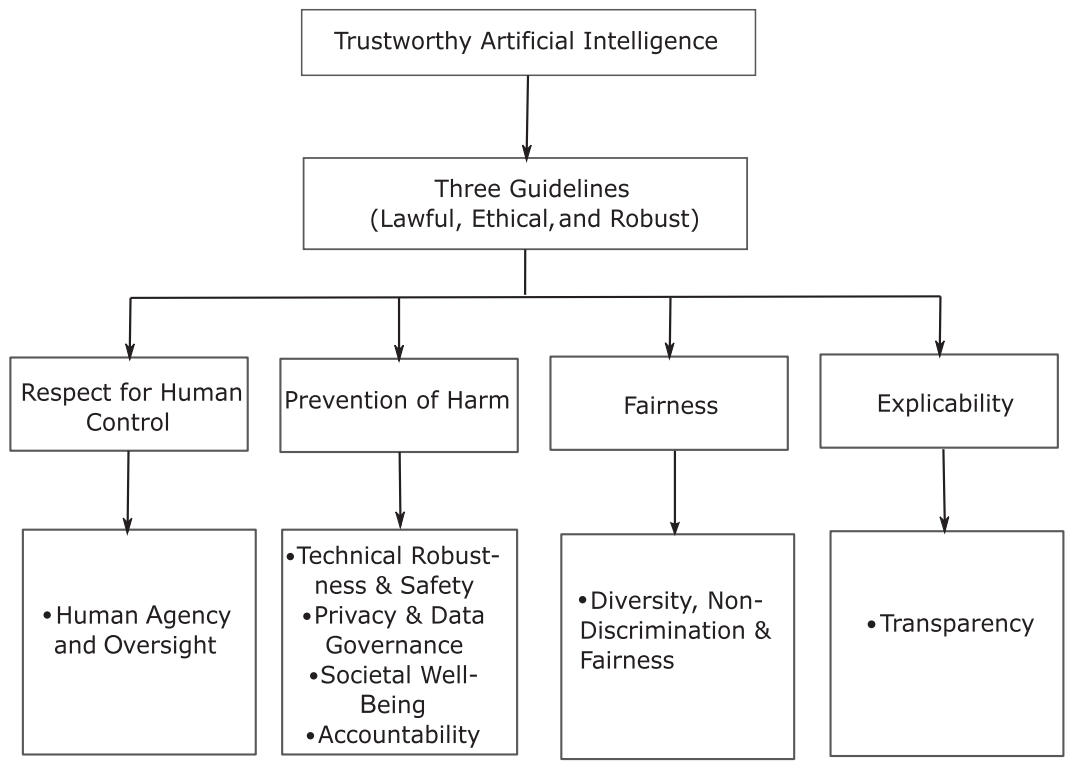
\includegraphics[width=0.8\linewidth]{Figures/TAI.png}
    \caption{Trustworthy AI framework~\cite{10.1145/3491209}}
    \label{fig:tai}
\end{figure}
%%%%%%%%%%%NEW DEB
\marginpar{Foundations of Trust}
From a conceptual perspective, trust is inherently linked to risk and vulnerability. In the organizational and behavioral sciences, trust is commonly defined as the willingness of a party to accept vulnerability to the actions of another under conditions of uncertainty and risk. In their seminal work, Mayer, Davis, and Schoorman formalize trust as the willingness of a trustor to be vulnerable to a trustee based on expectations regarding the trustee’s ability, benevolence, and integrity~\cite{55a601e8-f397-31d9-a222-5b5dd8d0bb15}. This definition emphasizes that trust is not merely a belief about expected outcomes, but a deliberate acceptance of potential negative consequences. It further distinguishes trust from related notions such as predictability or cooperation, which may exist without exposure to risk.

Beyond social and organizational contexts, the notion of trust has also been formalized in the domain of \ac{ICT} systems. In this setting, trust is not an abstract interpersonal concept but is defined as a relation between an agent and specific properties of a system, reflecting the agent’s belief that these properties hold within its perceived model of the system~\cite{10.1007/978-3-642-13446-3_14}. This perspective highlights two important aspects: first, trust is inherently subjective and depends on the agent’s knowledge and assumptions; second, trust is always tied to well-defined system properties, such as security guarantees or behavioral correctness.

\marginpar{Trust in Neural Networks}
These complementary perspectives provide a unified view of trust as both a risk-aware decision and an evidence-dependent relation to system properties. This conceptualization naturally extends to \ac{AI} systems. When a human user relies on the output of a \ac{NN}, for instance in medical diagnosis or automated decision-support, the user becomes vulnerable to errors, biases, and miscalibrated confidence estimates. At the same time, the user’s trust is implicitly grounded in assumptions about specific properties of the system, such as predictive reliability, robustness, and alignment with intended objectives. However, these properties are typically neither directly observable nor formally verifiable by the user.

Moreover, the internal decision-making processes of \acp{NN} are often opaque, limiting the user’s ability to monitor and validate individual predictions. As a result, reliance on such systems closely mirrors the trust relationships described in both organizational and formal \ac{ICT} settings: it involves accepting risk based on expectations about the system’s competence, reliability, and underlying assumptions. This dual nature of trust, as both vulnerability acceptance and property-based belief, highlights the need for formal, interpretable, and evidence-based approaches to trust assessment in \ac{NN} systems.

\marginpar{Limits of Current Metrics}
Despite this conceptual alignment, most existing approaches for evaluating \acp{NN} focus primarily on predictive performance metrics such as accuracy, precision, or recall. While these metrics are essential, they fail to capture whether a model is trustworthy in the sense required for high-stakes decision-making. A highly accurate model may still be unsafe if it is poorly calibrated, biased, or trained on unreliable data. Conversely, a model with lower predictive accuracy may be more trustworthy if it appropriately represents uncertainty and avoids overconfident predictions in unfamiliar or out-of-distribution scenarios.

Furthermore, trust in \acp{NN} is not solely a property of the model architecture or its learned parameters. It is inherently multi-layered and depends on the quality of the training data, the reliability of annotations, the behavior of the learning process, and the way uncertainty propagates from inputs to outputs. Dataset biases, labeling inconsistencies, and hidden correlations can undermine trust long before inference is performed. Without explicit mechanisms to assess and propagate trust across these components, users are left with opaque confidence scores that provide limited support for risk-aware decision-making.

These limitations motivate the need for a formal and interpretable framework for trust in \acp{NN}. Such a framework should explicitly represent uncertainty and support principled reasoning about how trust evolves as new information becomes available. It should also align with established theories of trust and risk, while remaining operational within modern \ac{ML} pipelines. This thesis addresses these requirements by grounding trust assessment in \acf{SL} and by developing mechanisms to quantify, propagate, and aggregate trust across datasets, network structures, and model outputs.


\subsection{Challenges in Quantifying Trust and Uncertainty in Neural Networks}
\label{sec:quantification_challenges}
Although the need for trust in \ac{NN} based systems is increasingly acknowledged, the quantification of trust and uncertainty remains an open and challenging problem. Unlike classical performance metrics, trust is not directly observable and cannot be measured through a single empirical quantity. Instead, it emerges from a combination of evidence, uncertainty, and risk, all of which must be represented in an interpretable manner.

A first challenge concerns the absence of a clear and unified definition of trust in the context of \acp{NN}. In practice, trust is often implicitly equated with predictive accuracy, confidence scores, or reliability estimates. However, these quantities capture only limited aspects of trust and do not account for the conditions under which a system may fail or behave unpredictably. Without a formal definition that distinguishes trust from related concepts, quantitative assessments remain inconsistent and difficult to assess across models and application domains.

A second challenge relates to the representation of uncertainty. Most \acp{NN} produce probabilistic outputs that are commonly interpreted as measures of confidence. However, such probabilities do not distinguish between uncertainty arising from insufficient evidence and uncertainty caused by conflicting evidence. For example, a prediction based on few training examples and a prediction derived from strongly disagreeing labels may both result in similar probability values, despite reflecting fundamentally different situations. This limitation complicates the interpretation of model outputs and limits their usefulness for risk-aware decision-making.

A third challenge lies in the quantification of trust at different levels of abstraction. Trust may be defined at the level of individual predictions, model components, datasets, or entire learning pipelines. Existing evaluation practices predominantly assess models at an aggregate level, relying on global performance metrics that obscure variation in trust and uncertainty across individual outputs. Consequently, predictions that are ambiguous or weakly supported by data are often treated equivalently to those that are well-supported. Addressing this limitation requires methods that can represent and evaluate trust at a finer granularity.

Another challenge concerns the integration of data quality into trust assessments. \acp{NN} are highly sensitive to the quality of training data, yet data-related issues such as labeling noise, annotator disagreement, and sampling bias are rarely incorporated into quantitative trust measures. In many cases, uncertainty introduced during data collection is not modeled and remains invisible at inference time. While these factors implicitly influence model behavior through training, their lack of explicit representation creates a disconnect that makes it difficult to reason about how much confidence should be placed in predictions derived from unreliable or contentious data.

Finally, there is a challenge associated with the propagation and aggregation of trust. In complex \ac{NN} architectures, trust assessments derived from different sources, such as data quality or component reliability, must be combined to form an overall judgment. Standard probabilistic frameworks offer limited support for such aggregation, particularly when sources of evidence are heterogeneous or partially dependent. Without principled operators for combining and propagating trust, quantitative assessments risk being inconsistent or misleading.

These challenges illustrate that quantifying trust and uncertainty in \acp{NN} requires more than probabilistic prediction and performance evaluation. It calls for representations that explicitly encode evidence, disagreement, and ignorance, and for reasoning mechanisms that support consistent propagation and aggregation of trust across system components. Addressing these challenges is the central objective of this thesis.

\section{Problem Statement and Research Questions}

This thesis aims to develop a formal, interpretable, and operational framework for assessing trust in \ac{NN} pipelines, both during training and inference. In particular, such framework should model how trust propagates from the training data to the learned model parameters, and from input observations to output predictions through the model. While traditional evaluation approaches primarily rely on predictive performance, they fail to capture essential aspects of trust such as uncertainty, incomplete knowledge, and the reliability of information sources. As \ac{NN} systems become increasingly complex and are deployed in safety-critical and open environments, these limitations become more pronounced.

To address this gap, this work investigates how trust can be modeled as an evidence-based quantity and systematically integrated across the different stages of the \ac{ML} system pipeline. In particular, the thesis explores how \ac{SL} can be adapted and used to represent, quantify, and combine trust in \ac{NN} systems. This includes assessing the trustworthiness of training datasets, modeling the propagation of trust through structured dependencies, and evaluating black-box models through observable signals such as calibration behavior.

The objective is therefore to provide a unified methodology that enables practical computation, interpretation, and use in real-world \ac{ML} systems. Based on these objectives and the challenges identified earlier, we formulate the following research questions.

\subsection{Part I: Efficient and Consistent Trust Inference with \aclu{SL}}
While \ac{SL} provides a formal and well-established framework for representing and combining uncertain information, its direct application to complex systems raises important challenges. In particular, performing trust inference over large and complex graphs can lead to significant computational overhead, as the number of operations required to propagate and aggregate opinions grows rapidly with the size and architecture of the system. This limits the scalability of existing approaches in realistic settings.

In addition to these computational challenges, existing \ac{SL} frameworks may lead to a loss of information during trust inference. In particular, successive transformations and unnecessary reduction operations can degrade the quality of the inferred trust values, resulting in less robust and less reliable trust quantification.

Finally, the process of propagating subjective opinions across such graphs may lead to inconsistencies, where the resulting trust assessments depend on the structure of the graph or the order in which operations are applied. This lack of stability undermines the reliability and interpretability of the inferred trust values.




These limitations restrict the applicability of \ac{SL} in complex systems where trust must be evaluated over interconnected components. Therefore, there is a need to define methods that reduce computational overhead, improve the robustness of trust quantification, and ensure the consistency of trust inference when applied to such settings.

This leads to the first research question:
\begin{rqbox}{Efficient and Consistent Trust Inference}
\label{rq:1}
    How can computational efficiency and consistency be ensured when performing trust inference with \ac{SL} over complex graphs?
\end{rqbox}


\subsection{PART II: Trustworthiness of Training Datasets}
Beyond the design of a formal framework for trust representation and propagation, trust in \ac{ML} systems is fundamentally influenced by the quality and reliability of the data used during training. In particular, training datasets serve as the primary source of evidence from which models learn, making their trustworthiness a critical factor in the overall behavior of the system.

However, existing approaches for dataset evaluation are often limited to statistical quality measures, bias detection metrics, or performance-based validation. While these methods provide useful insights, they do not offer a unified and interpretable way to quantify trust in datasets as an explicit function of evidence, uncertainty, and data reliability. Moreover, they typically fail to capture the impact of incomplete, noisy, or conflicting information, which is inherent in real-world data.

This creates a fundamental gap: although data is the foundation of learning, there is no framework to represent and quantify its trustworthiness in a way that is consistent with subsequent stages of trust assessment in the learning and inference processes. In particular, datasets are rarely modeled as structured sources of evidence that can be integrated into a broader trust reasoning framework.

Therefore, it is necessary to develop a method for assessing dataset trustworthiness that is both formally grounded and compatible with evidence-based trust modeling.

This leads to the second research question:
\begin{rqbox}{Trustworthiness of Training Datasets}
    How can the trustworthiness of training datasets be formally represented and quantified within an evidence-based framework?
\end{rqbox}

\subsection{PART III: Trust Propagation in \aclu{NN}s from Training Dataset to Inference}
Building upon the representation of trust and the quantification of dataset trustworthiness, a central challenge lies in understanding how trust propagates throughout the learning and inference processes. In \ac{ML} systems, trust is not confined to isolated components, but instead evolves across multiple stages, from the training data to the learned model parameters, and from input observations to output predictions.

During training, model parameters are inferred from data, implicitly inheriting the uncertainty, noise, and potential biases present in the dataset. Similarly, during inference, predictions are generated through complex transformations of the input, where uncertainty is accumulated and propagated throughout the model. Despite this, existing approaches typically assess trust at a single stage, either at the level of data, model performance, or output confidence, without providing a unified view of how trust flows across the entire pipeline.

This lack of continuity prevents a consistent interpretation of trust, as it remains unclear how uncertainties originating from the data influence the learned model, and how they subsequently affect predictions. Therefore, a key challenge is to establish a mechanism for modeling and quantifying the propagation of trust across both the learning and inference processes.

This leads to the third research question:
\begin{rqbox}{Trust Propagation from Training Dataset to Inference}
    How can trust be consistently propagated from training data to learned model parameters, and from inputs to outputs during inference, within an evidence-based framework?
\end{rqbox}
In practice, however, this assumption of full model transparency does not always hold, as many modern \ac{ML} models operate as black-box systems where internal parameters and intermediate computations are not accessible. While the propagation-based framework remains essential for understanding trust at a system level, this limitation motivates the need for complementary approaches that rely only on observable signals. This raises an important extension of the research question:
\begin{rqbox}{Trust Assessment under Limited Observability}
    how can trust be assessed when only observable data, such as model outputs are available?
\end{rqbox}



\section{Contributions of the Thesis}

This thesis introduces a unified and operational framework for trust assessment in \ac{ML} systems, with a particular focus on neural network pipelines. Building upon the research questions formulated in the previous section, the contributions of this work span the representation, quantification, and propagation of trust, as well as its practical evaluation in realistic settings. The main contributions are summarized as follows:

\begin{enumerate}
    \renewcommand{\labelenumi}{C\arabic{enumi}}
    \item \label{c:1}\textbf{A general methodology for trust assessment~\cite{5gaa_trust4cav_2025,connect_d31_taf}.}  
    This thesis proposes a \emph{General Trust Assessment Methodology} that formalizes trust as an evidence-based reasoning process. The methodology provides a structured framework for defining trust expressions, collecting and modeling evidence, and evaluating trust in a consistent and interpretable manner. It serves as a unifying backbone that can be instantiated across different components of a \ac{ML} pipeline.

    \item \label{c:2}\textbf{A scalable, consistent, and more robust framework for trust inference using Subjective Logic~\cite{10.1007/978-3-032-08887-1_4,10706345}.}  
    To address the limitations of applying \ac{SL} to complex systems, this work introduces methods that ensure computational efficiency, more robust trust quantification, and consistency of inference over large and complex graphs. In particular, it proposes an optimized graph analysis framework that enables stable, information-preserving, and scalable propagation of subjective opinions.

    \item \label{c:3}\textbf{A formal approach for assessing the trustworthiness of training datasets~\cite{ecmldatatrust,trust-aidatatrust}.}  
    This thesis develops a method to model training datasets as sources of evidence and to quantify their trustworthiness within an evidence-based framework. The approach captures uncertainty, noise, and potential biases in the data, allowing dataset quality to be explicitly integrated into the overall trust assessment process.

    \item \label{c:4}\textbf{A unified framework for trust propagation across learning and inference processes~\cite{patas}.}  
    A key contribution of this work is the formalization of trust propagation throughout the \ac{ML} pipeline. The proposed approach models how trust evolves from training data to learned model parameters, and from inputs to outputs during inference, providing a consistent and end-to-end view of trust in the system.

    \item \label{c:5}\textbf{A method for trust assessment in black-box models based on output data~\cite{11124121}.}  
    Recognizing that modern \ac{ML} systems often operate as black boxes, this thesis proposes an extension of the trust assessment framework that relies on observable quantities, such as calibration behavior. This enables the quantification of trust even when internal model information is not accessible, bridging the gap between theoretical modeling and certain practical deployment.
    
    \item \label{c:6}\textbf{An end-to-end evaluation on a real-world use case.}  
    The proposed framework is evaluated on a practical use case involving device energy consumption estimation. This evaluation demonstrates the applicability of the methodology in a realistic setting and highlights its ability to provide meaningful and interpretable trust assessments across the full pipeline.
\end{enumerate}
\begin{figure}
    \centering
    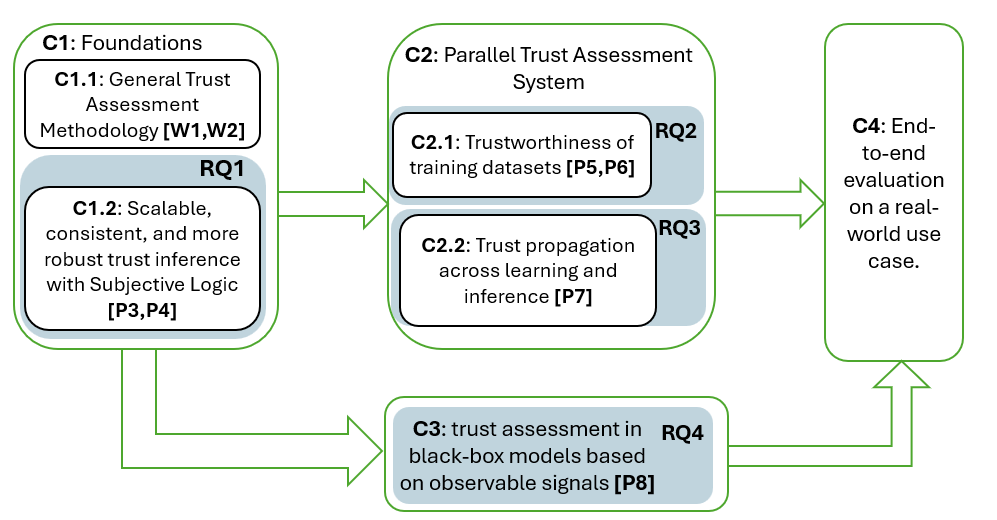
\includegraphics[width=0.9\linewidth]{Figures/contribution.png}
    \caption{overview of the main contributions of this thesis}
    \label{fig:contributions}
\end{figure}

\cref{fig:contributions} provides an overview of the main contributions of this thesis and their relationships. The contributions are organized into three conceptual layers, namely the foundations layer, the data and propagation layer, and the deployment layer. The figure highlights that the proposed General Trust Assessment Methodology (C\ref{c:1}) and the scalable trust inference framework (C\ref{c:2}) form the basis for subsequent developments, with (C\ref{c:2}) constituting a component of (C\ref{c:1}). It further illustrates that dataset trustworthiness (C\ref{c:3}) and trust propagation (C\ref{c:4}) are integrated within a unified pipeline, and that the general methodology extends to practical settings through black-box trust assessment (C\ref{c:5}) and the dataset trustworthiness assessment(C\ref{c:3}). Finally, it shows that both (C\ref{c:4}) and (C\ref{c:5}) extend to an end-to-end evaluation (C\ref{c:6}). The mapping to the research questions is also indicated, emphasizing the coherence between the problem formulation and the proposed contributions.



\section{Contributions of the Thesis}

This thesis proposes a unified and operational framework for trust assessment in \ac{ML} systems, with a particular focus on neural network pipelines. 
The contributions are structured into four main components, corresponding to the research questions and the different layers illustrated in \cref{fig:contributions}.

\subsection{Foundations: Trust Representation and Inference (C1)}

The first contribution establishes the theoretical and methodological foundations required to represent and reason about trust in complex systems. It is structured into two complementary sub-contributions addressing trust inference.

\textbf{C1.1 -- General Trust Assessment Methodology (\cref{chap:Trust_method})\cite{connect_d31_taf,5gaa_trust4cav_2025}.}  
This work introduces a general methodology for trust assessment based on evidence and structured reasoning. It formalizes trust as an explicit and interpretable process composed of (i) trust expression generation, (ii) atomic trust opinion quantification, and (iii) expression evaluation using \aclu{SL} operators. 
This contribution provides a domain-agnostic framework that serves as the backbone of all subsequent developments and addresses the need for a formal definition of trust in AI systems.

\textbf{C1.2 -- Scalable and Consistent Trust Inference Framework (\cref{chap:tnasl})~\cite{10.1007/978-3-032-08887-1_4}.}  
To enable the practical application of the methodology to complex systems such as \aclu{NN}, this thesis proposes an optimized trust inference framework. In particular, it introduces improved algorithms for Trust Network Analysis that ensure computational efficiency, reduce information loss, and guarantee consistency of inference results. This contribution directly addresses \textbf{RQ1} by enabling scalable and stable trust reasoning over complex dependency structures.

\subsection{Parallel Trust Assessment System (C2)}

The second contribution introduces a system-level framework that operationalizes trust assessment across the full \ac{ML} pipeline.

\textbf{C2 -- Parallel Trust Assessment System Overview (\cref{chap:ovl}).}  
This thesis proposes the \acf{PaTAS}, a framework that operates alongside \ac{NN} to assess trust without modifying their internal computations. \ac{PaTAS} provides a unified architecture that connects dataset trustworthiness, parameter reliability, and inference-time trust into a single coherent pipeline. It is structured around two main components: (i) a \emph{trust quantification layer}, which models trust in data and labels, and (ii) a \emph{trust propagation layer}, which mirrors \ac{NN} computations to propagate trust from dataset to model parameters during training and from inputs to outputs during inference.

\textbf{C2.1 -- Trustworthiness of Training Datasets (\cref{chap:data})~\cite{ecmldatatrust,trust-aidatatrust}.}  
A formal approach is developed to model datasets as structured sources of evidence and to quantify their trustworthiness using Subjective Logic. 
This contribution enables the assessment of dataset-level properties such as bias and reliability under uncertainty, including cases with incomplete or conflicting evidence. It directly addresses \textbf{RQ2} by providing a principled and interpretable framework for dataset trust quantification.

\textbf{C2.2 -- Trust Propagation Across Learning and Inference (\cref{chap:patas})~\cite{patas}.}  
Building on dataset trust, this work introduces mechanisms to propagate trust throughout the neural network, from training data to model parameters and from inputs to outputs during inference. 
The proposed PaTAS framework defines trust nodes and trust functions that mirror neural computations and enable end-to-end trust propagation.  
This contribution addresses \textbf{RQ3} by providing a consistent and operational solution for trust propagation across the entire ML lifecycle.

\subsection{Trust Assessment in Black-Box Models (C3)}

\textbf{C3 -- Trust Assessment under Limited Observability (\cref{chap:bb})~\cite{11124121}.}  
Recognizing that many real-world systems operate as black boxes, this thesis proposes a method to assess trust based solely on observable signals, such as model outputs and calibration behavior. 
This approach enables trust evaluation without access to internal model parameters or architecture, thereby extending the applicability of the framework to practical deployment scenarios.  
This contribution addresses \textbf{RQ4} by enabling trust assessment under limited observability.

\subsection{End-to-End Evaluation (C4)}

\textbf{C4 -- Real-World End-to-End Evaluation (\cref{chap:usecase}).}  
Finally, the proposed framework is validated through an end-to-end use case involving a real-world application. 
This evaluation demonstrates how the different components of the framework interact in practice and shows that the proposed approach provides meaningful, interpretable, and actionable trust assessments across the full AI pipeline.

\begin{figure}
    \centering
    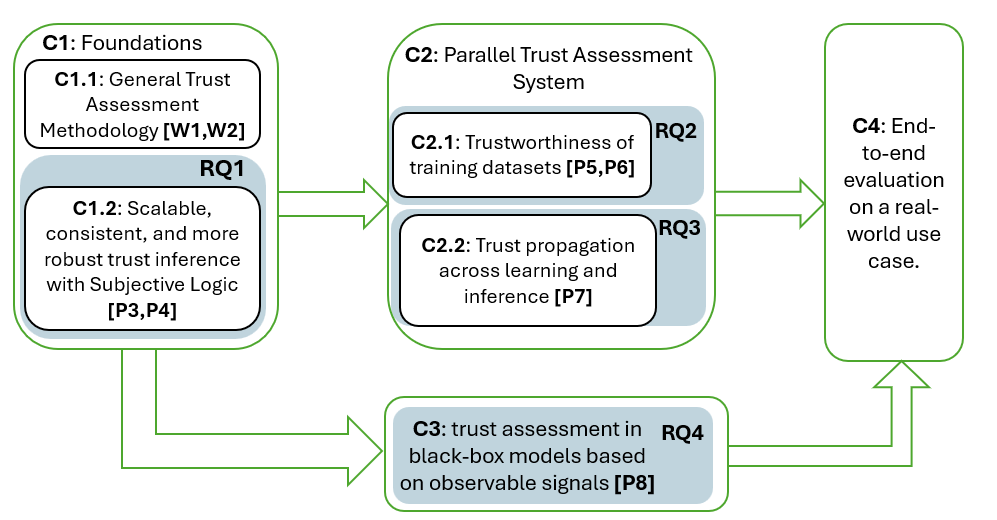
\includegraphics[width=0.9\linewidth]{Figures/contribution.png}
    \caption{overview of the main contributions of this thesis}
    \label{fig:contributions}
\end{figure}


Overall, these contributions form a coherent framework that enables the representation, quantification, propagation, and evaluation of trust in neural network systems. They collectively address the research questions defined in this thesis and provide both theoretical foundations and practical tools for trustworthy AI.

\cref{fig:contributions} presents an overview of the main contributions of this thesis and their relationships, structured according to the research questions. The contributions are organized into three conceptual layers: (i) the foundations layer (C1), (ii) the system and propagation layer (C2), and (iii) the deployment and evaluation layer (C3--C4).

At the foundation level, C1 establishes the theoretical and methodological basis for trust assessment. It combines a general trust assessment methodology (C1.1) with a scalable and consistent trust inference framework (C1.2), addressing \textbf{RQ1}. These components form the core building blocks upon which all subsequent contributions rely.

Building on these foundations, C2 introduces the Parallel Trust Assessment System, which operationalizes trust assessment across the machine learning pipeline. This component is decomposed into two complementary sub-contributions: dataset trustworthiness assessment (C2.1), addressing \textbf{RQ2}, and trust propagation across learning and inference (C2.2), addressing \textbf{RQ3}. Together, they form a unified pipeline that links data, model parameters, and predictions through consistent trust modeling and propagation.

In parallel, C3 extends the framework to settings where internal model information is not accessible. By relying solely on observable signals, it enables trust assessment in black-box models and addresses \textbf{RQ4}. This component complements the propagation-based approach by ensuring applicability of the methodology in black box deployment scenarios.

Finally, C4 integrates the different components into an end-to-end evaluation on a real-world use case. 
It demonstrates how trust can be assessed across the full pipeline, from data to inference, and validates the coherence and applicability of the proposed framework.



\section{Structure of the Thesis}

This dissertation is organized into several chapters that progressively develop a unified framework for trust assessment in \ac{NN} systems, spanning from theoretical foundations to practical instantiations across the \ac{NN} pipeline.

\cref{chap:rw} presents the theoretical foundations and related work. It reviews existing approaches for reasoning under uncertainty, including probabilistic methods, \aclu{DST}, and \ac{SL}. It also surveys prior work on trust and uncertainty in \acp{NN}, covering dataset quality and uncertainty quantification.The chapter concludes with a synthesis of the limitations of existing approaches, motivating the research questions addressed in this thesis.

\cref{chap:Trust_method} introduces the \emph{General Trust Assessment Methodology}, which forms the conceptual backbone of this dissertation. It formalizes trust as an evidence-based reasoning process structured around three main steps: (i) the generation of trust expressions through the decomposition of high-level trust propositions, (ii) the quantification of atomic trust opinions from available evidence, and (iii) the evaluation of these expressions using \ac{SL} operators. This methodology is designed to be domain-agnostic and serves as a unifying framework that forms the basis for all subsequent contributions.

\cref{chap:tnasl} focuses on the efficient and correct realization of the proposed methodology. It introduces an optimized \aclu{TNA-SL}, which enables the generation of trust expressions through structured graph-based representations. This chapter provides the theoretical and algorithmic foundation required to process complex graph in a consistent, robust and scalable manner.


\cref{chap:ovl} provides an overview of the \acf{PaTAS}, introducing a unified perspective on trust assessment across the different stages of the \ac{ML} pipeline. It presents the overall architecture of the proposed framework and outlines how trust can be analyzed from training data to model behavior during inference. In particular, this chapter identifies the key components involved in trust evaluation, including dataset-related factors, training processes, and inference mechanisms. It therefore serves as a system-level view that bridges the theoretical foundations and the subsequent detailed developments.



\cref{chap:data} instantiates the general methodology at the level of training data by addressing dataset trustworthiness. It focuses on the quantification of trust in datasets through properties such as labeling reliability and bias. Using \ac{SL}, the chapter treats datasets as structured sources of evidence and proposes methods to quantify their reliability, uncertainty, and potential biases
within an evidence-based framework. This chapter demonstrates how the proposed methodology can be applied to assess the reliability of data, which constitutes the foundation of any \ac{ML} system.

\cref{chap:patas} introduces the technical realization of the trust propagation layer within the \ac{PaTAS}. Building upon the dataset trustworthiness assessment, it integrates these inputs into the trust evaluation process and enables end-to-end computation of trust across the learning and inference stages. This chapter demonstrates how the different components of the framework interact in practice and how trust can be consistently propagated throughout the system.

\cref{chap:usecase} presents a use case illustrating the application of the proposed methodology in a real-world scenario. It demonstrates how trust can be assessed across different components of a system and highlights the practical relevance of the framework.

\cref{chap:bb} addresses the problem of trust assessment in black-box models. It proposes a calibration-based approach to quantify trust using observable signals, allowing trust evaluation when internal model information is not accessible. This chapter extends the work to support certain practical deployment settings.

Finally, \cref{chap:conclusion} summarizes the main contributions of the thesis and discusses limitations, perspectives, and directions for future work.












